\documentclass{book}

\usepackage{tesis_estilo}


\usepackage{graphicx}


\newcommand*{\titleGM}{\begingroup % Create the command for including the title page in the document
	\titlepage		% saco el número de página de la carátula
	\hbox{ % Horizontal box
		\hspace*{0.2\textwidth} % Whitespace to the left of the title page
		\rule{1pt}{\textheight} % Vertical line
		\hspace*{0.05\textwidth} % Whitespace between the vertical line and title page text
		\parbox[b]{0.75\textwidth}{ % Paragraph box which restricts text to less than the width of the page
			
			{\noindent\Huge\bfseries LTITOOL \\}\\[2\baselineskip] % Title
%			\begin{center}
				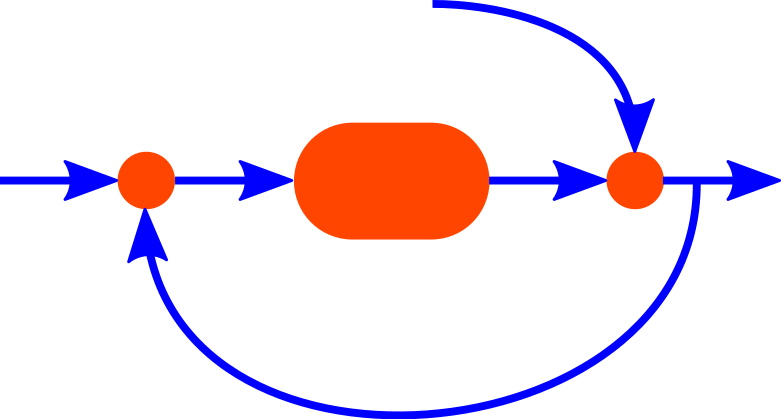
\includegraphics[scale=0.3]{./figuras/logos/logo_ltitool.png}
%			\end{center}
			
			
			{\large \textit{\\ LTI Control System Toolbox}}\\[4\baselineskip] % Tagline or further description
			{\large \textsc{ Eduardo J. Adam }} % Author name
			
			\vspace{0.5\textheight} % Whitespace between the title block and the publisher
			{\noindent \textsc{A\~{n}o:} \Year }\\[\baselineskip] % Publisher and logo
	}
	
    }
	
\textbf{Developers and Collaborators of this edition:}

\vspace{0.4cm}
\textsc{Eduardo J. Adam}, (\url{eadam.fiq@gmail.com})

Faculta de Ingeniería Química - Universidad Nacional del Litoral,

Santa Fe, Santa Fe, Argentina.


\vspace{2cm}
\textbf{Special thanks:}

\vspace{0.4cm}
Special thanks to Ernesto S. Burgos for the development of the GUI-Editor and for

for his selfless collaboration, which would otherwise it has made it impossible 

to achieve the GUIs here presented.

\vspace{0.2cm}
\textsc{Ernesto S. Burgos}, (\url{e.sergio.burgos@gmail.com})

Universidad Tecnoloógica Nacional - Facultad Regional Paraná,

Paraná, Entre Ríos, Argentina

.
	\endgroup}


% ------------
% New commands
% ------------
\def\Year{\expandafter\YEAR\the\year}
%\def\YEAR#1#2#3#4{#3#4}
\def\YEAR#1#2#3#4{#1#2#3#4}

% ----------------
% ---- macros ----
% ----------------






\begin{document}
\frontmatter
%\renewcommand{\tablename}{Tabla}
%\renewcommand{\listtablename}{Indice de tablas}
%\renewcommand\contentsname{Contenido}
%-----------------------------------------------------------------------
%Aqui va la carátula según reglamento de Maestría y Doctorado en Ingeniería Química y Tecnología Química
%-------------------------------------------------
%\titleGM	% Esta es la carátula definida arriba
%-------------------------------------------------
\titlepage

\begin{figure}
 \centering
 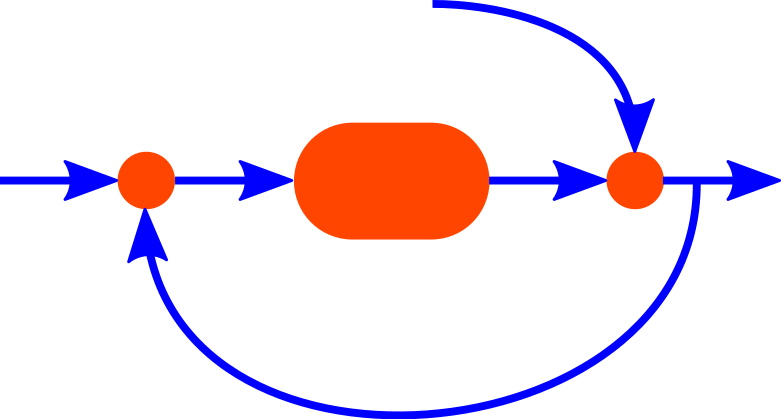
\includegraphics[scale=0.3]{./figuras/logos/logo_ltitool.png}
\end{figure}


\begin{center}
%\textbf{UNIVERSIDAD NACIONAL DEL LITORAL}

%\textbf{FACULTAD DE INGENIER\'IA QU\'IMICA}

\vspace{0.5cm}


\Large\textbf{LTI System Control Toolbox (LTITOOL)}


\vspace{1.5cm}
\normalsize{\textsc{Institution:}}

\normalsize{Cátedra de Instrumentación y Control de Procesos \\ Departamento de Ingeniería de Procesos -- FIQ -- UNL}



\vspace{1.5cm}
\textsc{Autor:}
\vspace{0.2cm}

\large{Prof. Dr. Eduardo J. Adam}
\vspace{0.1cm}

mailto: eadam.fiq@gmail.com

%\vspace{0.1cm}
%\url{http://www.fiq.unl.edu.ar/control/index.php?page=adam}

%\vskip 0.5cm
\vspace{0.5cm}
\vfill \textsc{A\~{n}o:} \Year
\end{center}

\newpage


\textbf{Developers and Collaborators of this edition:}

\vspace{0.4cm}
\textsc{Eduardo J. Adam}, (\url{eadam.fiq@gmail.com})

Faculta de Ingeniería Química - Universidad Nacional del Litoral,

Santa Fe, Santa Fe, Argentina.


\vspace{2cm}
\textbf{Special thanks:}

\vspace{0.4cm}
Special thanks to Ernesto S. Burgos for the development of the GUI-Editor and for

for his selfless collaboration, which would otherwise it has made it impossible 

to achieve the GUIs here presented.

\vspace{0.2cm}
\textsc{Ernesto S. Burgos}, (\url{e.sergio.burgos@gmail.com})

Universidad Tecnoloógica Nacional - Facultad Regional Paraná,

Paraná, Entre Ríos, Argentina


\tableofcontents

%-----------------------------------------------------------------------
\mainmatter
%A partir de aquí aparecen todos los capítulos numerados en el índice.

\chapter{Introduction} \label{Intro_chapter}
%\thispagestyle{fancy}

This particular toolbox is designed to facilitate the teaching, learning  and comprehension process of the linear control theory applyed to linear time invariant  (LTI) systems.

For this reason, this user manual makes use of classical theoretical concepts of linear control systems, based particularly on the work of Adam \cite{Adam2018}. \ footnote {Where the entire nomenclature is based on the cited text.}
 
This toolbox has 5 sections where the it is possible study
\begin{enumerate}
	\item Properties of open loop linear system as poles-zeros of transfer function and their relation to the dynamic responses to step and impulse.
	\item a first introduction to the analysis of linear systems with unit feedback, which includes pole and zero maps of the open and closed loop system, root locus, frequency analysis (Bode and Nyquist diagrams), 	dynamic responses of the feedback system to step set-point changes.
	\item 
	\item 
\end{enumerate}



				% INTRODUCCION
\chapter{Installation Mode} \label{Install_chapter}



\section{Installing for the First Time}
This toolbox are installed like any other Octave toolboxes. Consequently, the installation procedure is as detailed below.

\begin{enumerate}
	\item[\textbf{Step 1.}] Download the file \texttt{ltitool.tar.gz} To download the file for the first time you must go the website  \url{http://www.fiq.unl.edu.ar/control/index.php?page=software}.
	\item[\textbf{Step 2.}] Run the following command in the directory where the file was downloaded.
	\begin{verbatim}
		>>> pkg install ltitool.tar.gz
	\end{verbatim}
\end{enumerate}

In this way, the toolbox is already installed and ready to use. Then, write the following commands to execute the toolbox mentioned before:
	\begin{verbatim}
		>>> pkg load ltitool
		>>> ltitool
	\end{verbatim}

\section{Updating the Version}

If you already have LTITOOOL installed, then when a new version is available, a window like the one is shown in Fig. \ref{chp_install_fig01}.

\begin{figure}[H]
	\centering
	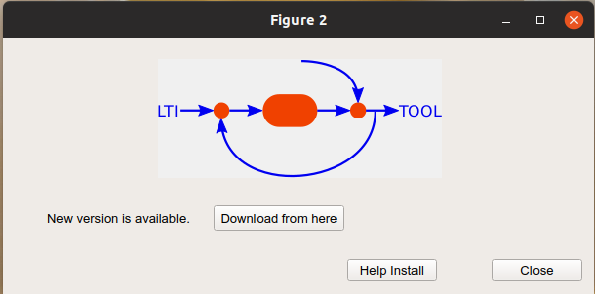
\includegraphics[scale=0.58]{./figuras/chapter_install/ltitoolNewVersionWnd.png}
	\caption{Updating to a new version.}
	\label{chp_install_fig01}
\end{figure}



Simply, you have to press the download button and then you have to follow the procedure indicated  below.
\begin{enumerate}
	\item[\textbf{Step 1.}] Uninstall the version you currently have installed. To do this, execute the command
	\begin{verbatim}
		>>> pkg uninstall ltitool.tar.gz
	\end{verbatim}
	Alternatively, it might be convenient to close and reopen Octave, but this should not be necessary.

	\item[\textbf{Step 2.}] Run the following command in the directory where the file was downloaded.
	\begin{verbatim}
		>>> pkg install ltitool.tar.gz
	\end{verbatim}
	
	Finally, you have the new version installed and to execute it you must follow the steps indicated in the previous section.
\end{enumerate}


 			% Instalación

\chapter{Open Loop LTI Systems} \label{LA_chapter}

The transient response analysis carried out in this chapter is based on using a representation with  transfer functions of the system output according to his input. The use of this particular representation is more intuitive for the process engineer, since it consists of a simple input-output representation, where if it take into account that for its study the input has been set a priori, the transient output can predicted immediately from the analysis of the system transfer function.

\vspace{0.4cm}
To do this, consider the open loop system of the Fig. \ref{chp_la_fig01_la}.

\begin{figure}[H]
	\centering
	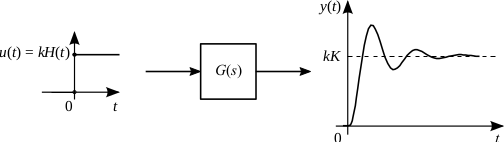
\includegraphics[scale=1.2]{./figuras/chapter_gla/fig_la.png}
	\caption{Open loop LTI system}
	\label{chp_la_fig01_la}
\end{figure}
where \textit{Y}(\textit{s}) = \textit{G}(\textit{s})\textit{U}(\textit{s}) with \textit{G}(\textit{s}) a polynomial ratio written as,

\begin{equation}\label{eqn01_chp_la}
	G(s)=\frac{b_m s^m \dots b_1 s + b_0}{s^n+a_1s^{n-1}+\dot a_{n-1}s^1 + a_n}
\end{equation}

Note that the dynamic response turns out to be,
\begin{equation}\label{eqn02_chp_la}
	y(t)= \mathscr{L}^{-1} \left[ \frac{b_m s^m \dots b_1 s + b_0}{s^n+a_1s^{n-1}+\dot a_{n-1}s^1 + a_n} U(s)\right]
\end{equation}
where the available inputs in this application are step and impulse.


\section{Impulse response}\index{inpulse!response}

Impulse response \index{impulse response} is the system dynamic response subjected to the input signal equal to a Dicrac delta input (denote as $\delta(t)$).

Thus, being the temporary expression of an unit impulse $u(t) = \delta(t)$, its Laplace transform results $U(s) = \mathscr{L}[u(t)] = \mathscr{L}[\delta(t)] = 1$ then,  \textit{Y}(\textit{s}) = \textit{G}(\textit{s}) and the dynamic LTI system response is,

\begin{equation} \label{Eq06_chp_trans}
y(t) = \mathscr{L}^{-1}[G(s)] ~~\mbox{.}
\end{equation}

In conclusion, \textit{the impulse response of a linear system is equal to the inverse transformation of its plant transfer function.}

\vspace{0.4cm}
\textbf{Example 1} \label{ejem01_gla_oct}

%\begin{example} \label{ejem01_gla_oct}
	Consider a linear system whose transfer function is,
	\begin{equation}\label{eqn_Gs_ejem01}
		G(s)=\frac{(s+1)}{s^2+ 0.5 s +1}
	\end{equation}
	subject to a Dirac Delta input. We pretend to obtain the dynamic system response  subject to such excitation.
	
	\vspace{0.4cm}
	To do this, before carrying out a simulation, we will make a study based on the transfer function of the system.
	
	\vspace{0.4cm}
	\begin{enumerate}
		\item \textbf{Stability:} It is possible to determine this based on the poles of the system transfer function, in this case under open loop. To do this, using Octave, you can determine these poles using the following commands:
		
		\vspace{0.4cm}
		%------------------------------------------------------------------------------------------------------
		% Cargo archivo de Octave para motrar en el ejemplo
		%\lstinputlisting[language=Octave,frame=single,firstline=6, lastline=16, caption=Código de Octave del Ejem. \ref{ejem01_gla_oct} para el calculo de las raíces de lazo cerrado.]{./m/chapter_la/ejem01_ltitool.m}
		%------------------------------------------------------------------------------------------------------
		
		\begin{verbatim}
		% System transfer function
		s=tf('s');
		Gs=(s+1)/(s^2+0.5*s+1);
		
		% Poles and Zeros
		polesGs=roots(Gs.den{1,1})
		\end{verbatim}
		
		\vspace{0.4cm}
		La respuesta en la ventana de comandos de Octave es:
		\begin{verbatim}
		polesGs =
		
		-0.25000 + 0.96825 i
		-0.25000 - 0.96825 i
		\end{verbatim}
		
		\item \textbf{Initial and Final Value:} These values can be determined by the initial (IVT) and final (FVT) values theorems.
		
		\vspace{0.4cm}
		Taking into account the following remark:
		
		\begin{remark}
			\begin{remarca}\label{rem01_chp_trans}
				The initial value ($t = 0^+$) of the impulse response of the self-regulating linear system itself with \textit{n} > \textit{m} is a finite magnitude.
			\end{remarca}
			
			\begin{demo}
				See Adam's textbook \cite{Adam2018}, among others.
			\end{demo}
		\end{remark}
	
	    Where it is denoted as \textit{n} the denominator polynomial order and \textit{m} that corresponding to the numerator.
		
		\vspace{0.4cm}
		According to IVT,
		
		\begin{eqnarray*}
			y(0^{+}) &=& \lim _{s \to \infty } sG(s)U(s)\\
			&=& \lim _{s \to \infty } s \frac{(s+1)}{\left ( s^2 + 0.5 s + 1 \right ) } 1\\
			&=& 0  ~~\mbox{.}
		\end{eqnarray*}
		
		\vspace{0.4cm}
		
		\begin{remark}
			\begin{remarca}\label{rem02_chp_trans}
				The final value ($t \to \infty$) of the impulse response of a self-regulating linear system itself with $n \ge m$ is zero.
			\end{remarca}
			
			\begin{demo}
				See Adam's textbook \cite{Adam2018}, among others.
			\end{demo}
		\end{remark}
		
		According to FVT,
		
		\begin{equation*} 
			y(\infty)= \lim _{s \to 0} s Y(s) = \lim _{s \to 0} s G(s)U(s) = \lim _{s \to 0} s \frac{(s+1)}{s^2+0.5 s+1}1=0
			~~\mbox{.}
		\end{equation*}
		
		
		\item \textbf{Impulse Response:} With the previously information it is possible to predict the system dynamic behavior. For this particular case, we can predict that the system leaves zero (through the IVT) and returns to zero (through the FVT). In addition, it will oscillate around the final value since such system has two complex conjugate roots, according to previous calculations.
		
		
		Also, using the \texttt{impulse}  Octave command you can determine the dynamic open-loop response of the system for a Dirac delta input, as indicated below.
		
		\begin{verbatim}
		% System transfer function
		s=tf('s');
		Gs=(s+1)/(s^2+0.5 s+1);
		
		% Impulse response
		impulse(Gs)
		\end{verbatim}
		obtaining the following graph:
		
		\begin{figure}[H]
			\centering
			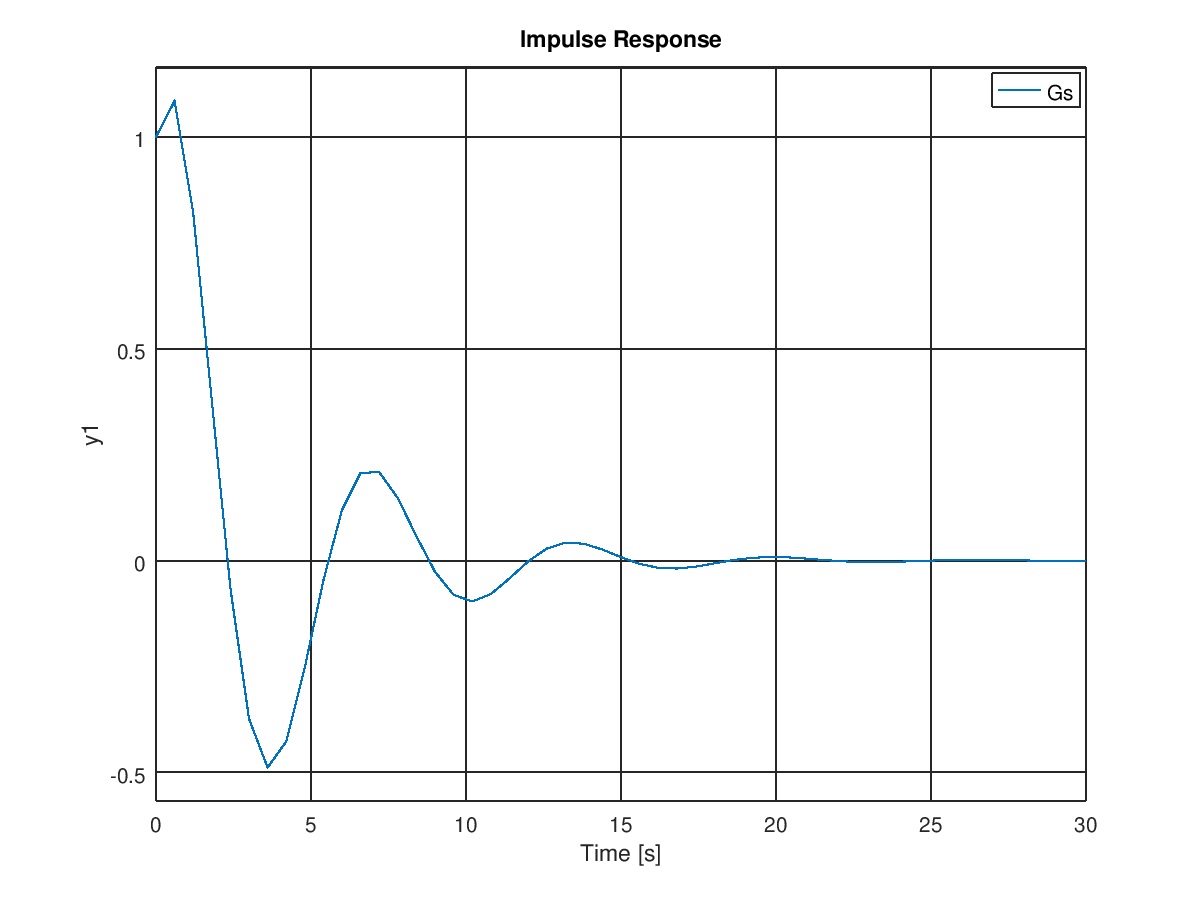
\includegraphics[scale=0.55]{./m/chapter_la/impulseGs_ltitool.png}
			\caption{System impulse response (\ref{eqn_Gs_ejem01}).}
			\label{chp_la_fig02_impulse}
		\end{figure}
		
	\end{enumerate}
	
%\end{example}



\section{Step response}\index{step!response}

Now, consider the system dynamic response subjected to a step input signal with amplitude \textit{k}.

The step temporal expression is, \textit{u}(\textit{t}) = \textit{kH}(\textit{t}) where, \textit{H}(\textit{t}) is the Heavyside function and therefore, the Laplace transform of \textit{u}(\textit{t}) is \textit{U}(s) = \textit{k}/\textit{s}.  Consequently, the temporal response of the linear system results,

\begin{equation} \label{Eq08_chp_trans}
y(t) =  \mathscr{L}^{^-1} \left[G(s) \frac{k}{s}  \right]   ~~\mbox{.}
\end{equation}

That is to say: \ textit {the step response with amplitude \textit{k} of a linear system is equal to the inverse Laplace transform of the transfer function multiplied by \textit{k}/\textit{s}.}

\vspace{0.4cm}
\textbf{Example 2} \label{ejem02_gla_oct}

%\begin{example} \label{ejem02_gla_oct}
	Consider a linear system of the Exam. \ref{ejem01_gla_oct} whose transfer function is given by (\ref{eqn_Gs_ejem01}). Obtain the dynamic response of such system for a step input.
	
	\vspace{0.4cm}
	Firstly, it is studied
	
	\vspace{0.4cm}
	\begin{enumerate}
		\item \textbf{Stability:} This depends on the roots of the characteristic equation and is not affected by the type of input. Therefore, the system will have a stable open loop dynamic response for the step input.
		\item \textbf{Initial and Final Values:} They can be determined by IVT and FVT. 
		
		For IVT, the following remark is established below.
		
		\begin{remark}
			\begin{remarca}\label{rem03_chp_trans}
				The initial value of the step response of the self-regulating linear system itself is zero if \textit{n} > \textit{m} and nonzero if \textit{n} = \textit{m}.
			\end{remarca}
			
			\begin{demo}
				See Adam's textbook \cite{Adam2018}, among others.
			\end{demo}
		\end{remark}
		
		According to Eq. (\ref{eqn_Gs_ejem01}), it is easy to proof that,
		\begin{equation*} 
			y(0^+)= \lim _{s \to 0} s Y(s) = \lim _{s \to 0} s \ G(s)U(s) =  \lim _{s \to \infty} \cancel{s} \frac{(s+1)}{s^2+0.5s+1} \frac{k}{\cancel{s}} = 0 ~~\mbox{.}
		\end{equation*}
		
		
		For FVT, the following remark is established below.
		
		
		\begin{remark}
			\begin{remarca}\label{rem04_chp_trans}
				The final value of the step response of the self-regulating linear system itself is equal to \textit{kK}.
			\end{remarca}
			
			\begin{demo}
				See Adam's textbook \cite{Adam2018}, among others.
			\end{demo}
		\end{remark}
	
		Where it is denoted as \textit{k} the step amplitude  and \textit{K} to the static gain \index{static gain} of the open loop plant.
		
		\vspace{0.4cm}
		According to the FVT and taking into account Eq. (\ref{eqn_Gs_ejem01}) it is possible to write,
		
		\begin{equation*} 
			y(\infty)= \lim _{s \to 0} s Y(s) = \lim _{s \to 0} s \ G(s)U(s) = \lim _{s \to 0} \cancel{s} \frac{(s+1)}{s^2+0.5s+1} \frac{k}{\cancel{s}} =  k
		\end{equation*}
		
		\item \textbf{Step response:}
		With the previously determined information, the system dynamic behavior  can be predicted for the amplitude input step \textit{k}. For this example particular, it can be predicted that the system leaves zero (IVT) and reaches a final value equal to \textit{kK} (FVT). In addition, the dynamic response will oscillate around the final value since such system has two complex conjugate roots, according to  previously calculus.
		
		
		In addition, using the Octave command \texttt{step} , the dynamic open loop response of the system can be determined, as indicated below.
		
		\begin{verbatim}
		% System transfer function
		s=tf('s');
		Gs=(s+1)/(s^2+0.5*s+1);
		
		% Step response
		step(Gs)
		\end{verbatim}
		
		Thus the Fig. \ref{chp_la_fig03_step} is obtained.
		
		\begin{figure}[H]
			\centering
			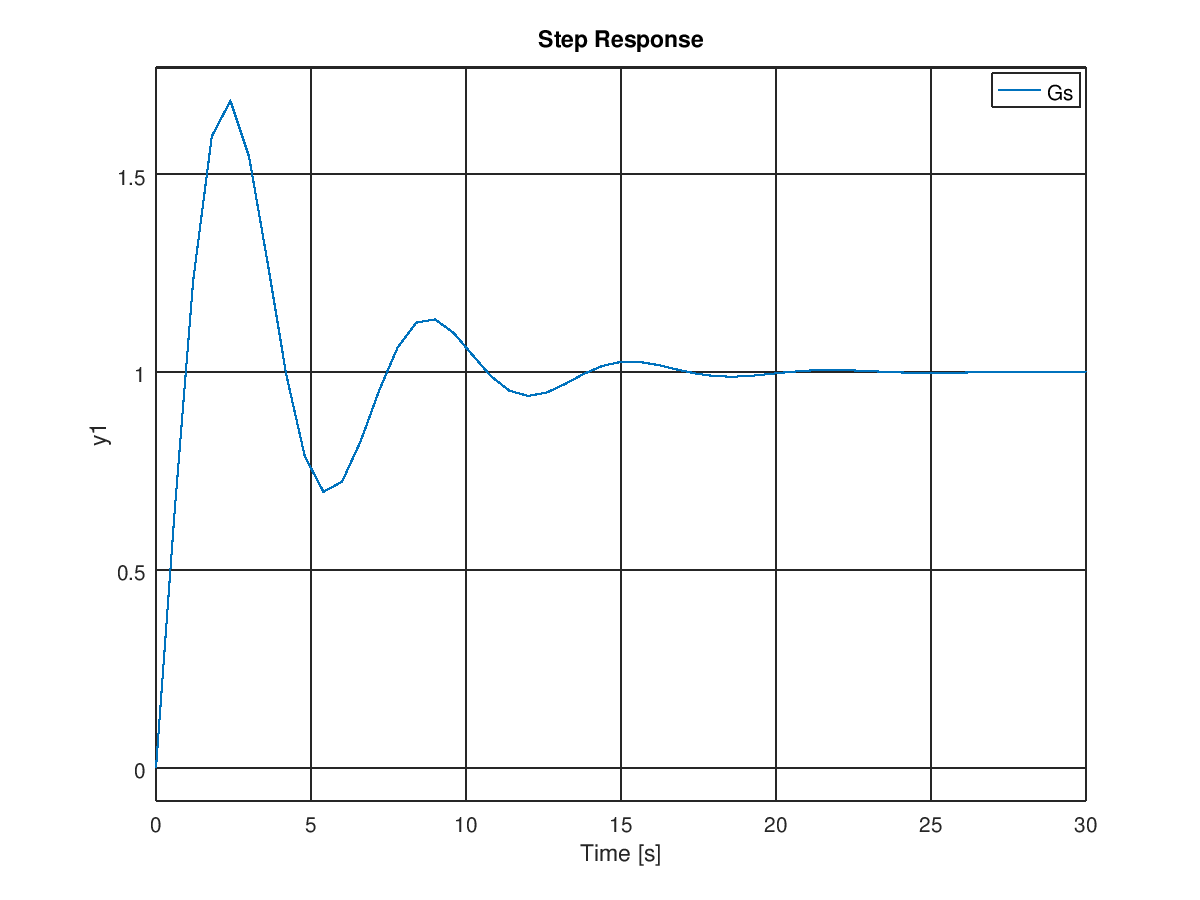
\includegraphics[scale=0.55]{./m/chapter_la/stepGs_ltitool.png}
			\caption{System step response (\ref{eqn_Gs_ejem01}).}
			\label{chp_la_fig03_step}
		\end{figure}

	\end{enumerate}



%\end{example}


\section{Tool Developed for Open Loop Systems}

This tool allows:
\begin{enumerate}
	\item To determine poles and zeros maps of a transfer function.
	\item Similarly, impulse and step dynamic responses of \textit{G}(\textit{s}) are presented in the main application window. Also, it is necessary to specify,
	\begin{enumerate}
		\item step amplitude, in case of choosing for this option and
		\item simulation time.
	\end{enumerate}
\end{enumerate}

Also in this developed tool additional information is presented, as
\begin{enumerate}
	\item Stability or instability of the LTI system.
	\item Final value reached by the open loop system once the transient has finished.
	\item Approximate settling time, which is calculated based on the dominant poles of the system. Such calculus can be improved if the simulation time is extended.
\end{enumerate}

\vspace{0.4cm}
\textbf{Example 3}

It is pretend to obtain the open-loop response to the step and delta for the transfer function,
\begin{equation}
	G(s)=\frac{s+1}{s^2+0.5s+1}
\end{equation}
the application can be invoked in command mode as indicated below.

\begin{verbatim}	
	% packages are loaded.
	pkg load control signal ltitool
	
	% Clean memory and command window.
	clear all, clc
	
	% Complex variable  "s"
    s = tf("s");
    % plant
    Gol=(s+1)/(s^2+0.5*s+1);
    % simulation parameters
    k=1;        % step amplitude
    tFinal=20;  % simulation time


   % ------------------------------------------------------------------------
   % Poles-Zeros Map
   % ------------------------------------------------------------------------
   title_string='Poles and Zeros Map of G(s)';
   legend_zeros_string='Zeros of G(s)';
   legend_poles_string='Poles of G(s)';

   figure(1), 
   xpzmap(title_string,legend_zeros_string,legend_poles_string, ... 
   Gol.num{1,1},Gol.den{1,1});

   % ------------------------------------------------------------------------
   % Simulation
   % ------------------------------------------------------------------------
   % Step response
   figure(2), OLstepresponse(Gol.num{1,1},Gol.den{1,1},k,0.0,tFinal,1000);

   % Impulse response 
   figure(3), OLimpulseresponse(Gol.num{1,1},Gol.den{1,1},0.0,tFinal,1000);

   % ------------------------------------------------------------------------
   % Additional information 
   % ------------------------------------------------------------------------
   [stability,yinf,Test]=additionalinfo(Gol.num{1,1},Gol.den{1,1}, ...
                                       tFinal,1000)
\end{verbatim}

The command window reports
\begin{verbatim}
>> stability = Asympt. Stable
>> yinf =  1
>> Test =  16.060
\end{verbatim}


Notice that in the case of the step response, the command window reports that \texttt{yinf=1}while for the impulse response \texttt{yinf=0}.

\vspace{0.4cm}
\textbf{Example 4}

The same example can be solved directly by invoking the analysis and simulation window  of open-loop linear systems, simply by typing in the command window,
\begin{verbatim}
>> pkg load control signal ltitool,
>> oLWnd;
\end{verbatim}
and then Octave will present the window that it shows in Fig. \ref{chp_la_fig01_GLA}.

\begin{figure}[H]
	\centering
	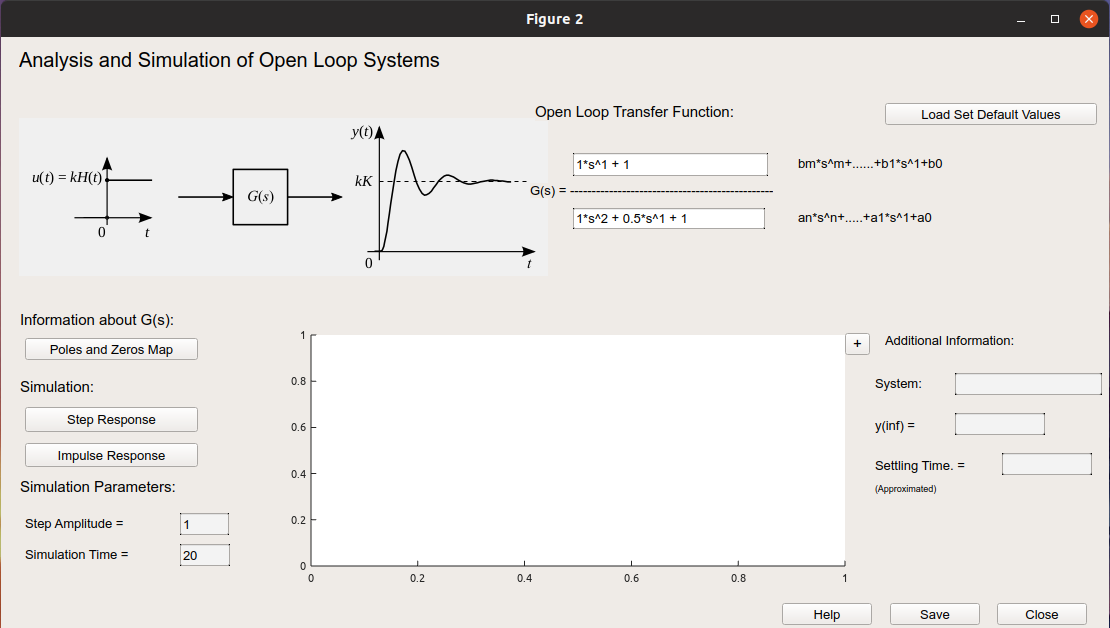
\includegraphics[scale=0.5]{./figuras/chapter_gla/fig01_ejemGLA.png}
	\caption{Analysis and simulation window for LTI systems in open loop.}
	\label{chp_la_fig01_GLA}
\end{figure}

Notice that, 
\begin{itemize}
	\item The window has preloaded data that can be changed.
	\item It is possible to specify, step amplitude and simulation time.
	\item It can be obtained easily  (i) poles-zeros map, (ii) step response or, (iii) impulse response.
	\item The + button throws a graph out of the application window.
\end{itemize}

\vspace{0.4cm}
By way of example, the Fig. \ref{chp_la_fig02_GLA} shows the step response along with the additional  information about stability, reached steady state value and settling time.

\begin{figure}[H]
	\centering
	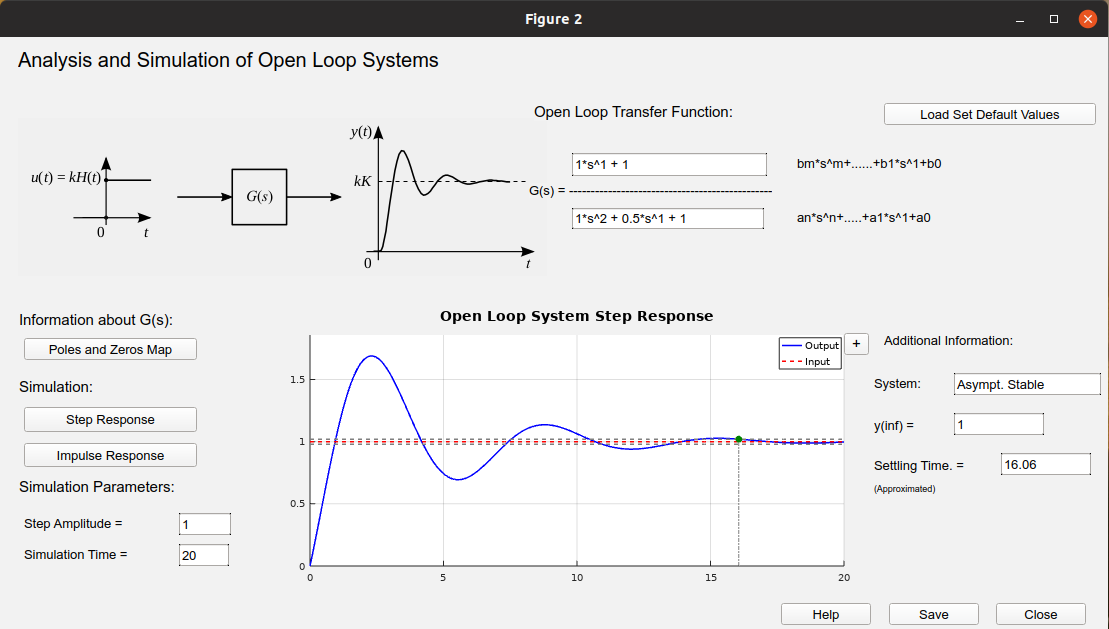
\includegraphics[scale=0.5]{./figuras/chapter_gla/fig02_ejemGLA.png}
	\caption{Open loop LTI system analysis and simulation window after pressing the step response button.}
	\label{chp_la_fig02_GLA}
\end{figure}



\section{Conclusions}

				% Sistemas a Lazo Abierto

\chapter{Closed Loop LTI Systems} \label{lc_chapter}
%\thispagestyle{fancy}

Consider the closed loop system given by Fig. \ref{chpCLfig01Gcl}.

\begin{figure}[H]
	\centering
	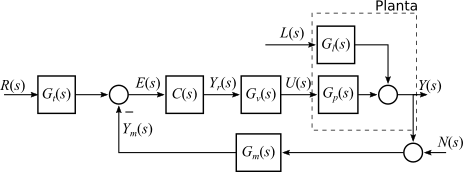
\includegraphics[scale=1.2]{./figuras/chapter_glc/lazocerrado.png}
	\caption{Closed loop LTI system.}
	\label{chpCLfig01Gcl}
\end{figure}


The closed loop system given by Fig. \ref{chpCLfig01Gcl} can be redrawn as presented in Fig. \ref{chp_lc_fig02_GH} for a setpoint change where, according to Adam \cite[see Chap. 9]{Adam2018}, if $G_t(s)=G_m(s)$ the feedback system has a similar behavior that a unity feedback system and consequently it is possible to write, $G(s)=G_p(s)G_v(s)G_m(s)$ y \textit{H}(\textit{s})=\textit{C}(\textit{s}).
\begin{figure}[H]
	\centering
	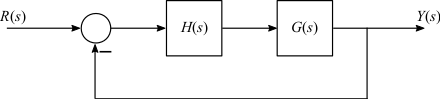
\includegraphics[scale=1.2]{./figuras/chapter_glc/fig_GH.png}
	\caption{Closed loop LTI system with unity feedback.}
	\label{chp_lc_fig02_GH}
\end{figure}

For the stability study, remember that it must take into account (Adam, \cite{Adam2018}):

\begin{theorem}[Routh-Hurwitz stability Criterion] \label{teo02_chp_estab}\index{stability!Routh-Hurwitz criterion}
	The necessary and sufficient condition of stability is that all the terms in the first column of the Routh array have the same sign.
\end{theorem}

In this toolbox version, two tools have been developed to allow studying of  stability by mean of the root locus and  Bode and Nyquist stability criteria.

\vspace{0.4cm}
\textbf{Example 3.1.} \label{ejem01_gh_oct}
%\begin{example} \label{ejem01_gh_oct}
Firstly, consider a unity feedback system whose transfer function is presented in Fig. \ref{fig01_ejem01_GH}, with a PI controller where $K_r$ is a variable gain and $T_I=5$. 
\begin{figure}[H]
	\centering
	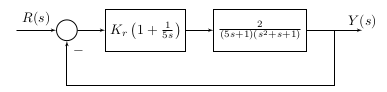
\includegraphics[scale=1.2]{./figuras/chapter_glc/fig_GH_ejem01.png}
	\caption{Unity feedback system given by Exam. 1.}
	\label{fig01_ejem01_GH}
\end{figure}

The open loop transfer function, \textit{G}(\textit{s})\textit{H}(\textit{s}) results,

\begin{equation}\label{eqn01_ejem01_lc}
	G(s)H(s)=\frac{K_r\cancel{(5s+1)}}{5s}\frac{2}{\cancel{(5s+1)}(s^2+s+1)}=\frac{K^*}{s(s^2+s+1)}
\end{equation}

where for this particular case $K^*=2K_r/5$.

\vspace{0.4cm}
For this example, the closed loop transfer function results,

\begin{equation}\label{eqn02_ejem01_lc}
	\frac{Y(s)}{R(s)}=G_{lc}(s)=\frac{G(s)H(s)}{1+G(s)H(s)}=\frac{K^*}{s^3+s^2+s+K^*}.
\end{equation}

To study the stability of the feedback system,  the Routh stability criterion will be apply based on the characteristic equation of feeback loop system.

Being the characteristic equation of this example, $D(s)=s^3+s^2+s+K^*$ and therefore the Routh array results

\begin{equation*}
	\begin{array} {c|}
		s^3 \\ s^2 \\ s^1 \\ s^0
	\end{array}
	\begin{array} {cc}
		1  & 1 \\
		1  & K^* \\
		1-K^*  & 0  \\
		K^*  & 0 \\
	\end{array}
\end{equation*}

It follows that the system will be \textit{asymptotically stable} if and only if, 0 < \textit{K}* < 1.

\vspace{0.4cm}
Now it is pretended to study the initial and final values reached for a step change in the setpoint \textit{R}(\textit{s}) = \textit{k/s}. To do this, applying the initial value theorem (IVT),
\begin{equation*} 
	y(0^+)= \lim _{s \to \infty} s Y(s) = \lim _{s \to \infty} s \ G_{lc}(s)R(s) =  \lim _{s \to \infty} \cancel{s} \frac{K^*}{s^3+s^2+s+K^*} \frac{k}{\cancel{s}} = 0 ~~\mbox{.}
\end{equation*}

Then, applying the final value theorem (FVT),
\begin{equation*} 
	y(\infty)= \lim _{s \to 0} s Y(s) = \lim _{s \to 0} s \ G_{lc}(s)R(s) = \lim _{s \to 0} \cancel{s} \frac{K^*}{s^3+s^2+s+K^*} \frac{k}{\cancel{s}} =  k
\end{equation*}

From the results of both theorems it is shown that the system starts from zero and reaches the setpoint value. This result is subject to the system being stable in closed loop; this is, 0 < \textit{K}* < 1.

\vspace{0.4cm}
Now adopting \textit{K*} = 0.5 (o sea \textit{Kr} = 1.25) to reach a \textit{GM} = 2, the characteristic closed loop equation results $D(s)=s^3+s^2+s+0.5$ presenting three poles in $s_1= -0.64780$ y $s_{2-3}=-0.17610 \pm j 0.86072$.

Note that both systems do not have zeros.

\vspace{0.4cm}
These results can be easily obtained with the Octave commands,
%------------------------------------------------------------------------------------------------------
% Cargo archivo de Octave para motrar en el ejemplo
%\lstinputlisting[language=Octave,frame=single,firstline=9, lastline=20, caption=Código de Octave del Ejem. \ref{ejem01_glc_oct} para el calculo de las raíces $G(s)H(s)$ y de $G_{lc}(s)$.]{./m/chapter_la/ejem01_lc_ltitool.m}
%------------------------------------------------------------------------------------------------------

\begin{verbatim}
    pkg load control
    
	% G(s)H(s) transfer function
	Kast=0.5;
	s=tf('s');
	GH=Kast/(s*(s^2+s+1));
	
	% G(s)H(s) Poles-Zeros
	polesGH=roots(GH.den{1,1})
	% Closed loop Poles-Zeros
	Gcl=feedback(GH,1)
	polesGcl=roots(Glc.den{1,1})
\end{verbatim}

where the answer in the Octave command window is,
\begin{verbatim}
	polesGH =
	
	-0.50000 + 0.86603i
	-0.50000 - 0.86603i
	0.00000 + 0.00000i
	
	
	Transfer function 'Glc' from input 'u1' to output ...
	
	           0.5
	y1:  -------------------
	     s^3 + s^2 + s + 0.5
	
	Continuous-time model.
	polesGcl =
	
	-0.17610 + 0.86072i
	-0.17610 - 0.86072i
	-0.64780 + 0.00000i
\end{verbatim}

The feedback system step response can be obtained by means of the following Octave command:
\begin{verbatim}
	% Step response
	step(Glc)
\end{verbatim}
that it shown in Fig. \ref{chp_lc_fig01_step_GH}.
\begin{figure}[H]
	\centering
	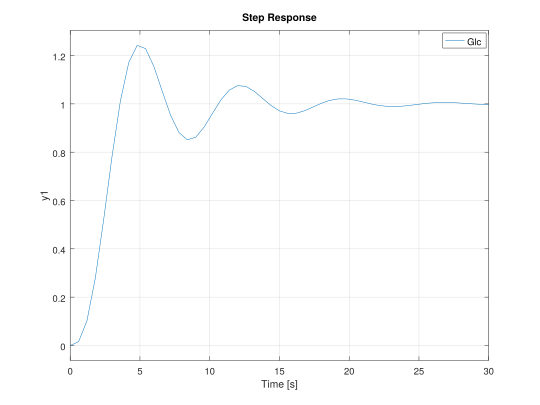
\includegraphics[scale=0.85]{./figuras/chapter_glc/fig01_step_lc.png}
	\caption{Unit step response of the feedback system of the Fig. \ref{fig01_ejem01_GH}.}
	\label{chp_lc_fig01_step_GH}
\end{figure}
%\end{example}



\section{Tools for Feedback LTI Systems}

As mentioned before, two tools for the analysis and simulation of closed loop LTI systems were developed. These ones apply to 
\begin{enumerate}
	\item Feedback system based on \textit{G}(\textit{s})\textit{H}(\textit{s}) according to Fig. \ref{chp_lc_fig02_GH} and,
	\item Closed loop system under the representation of \ref{chp_lc_fig01_lc}.
\end{enumerate}

\subsection{Analysis and Simulation Based on \textit{G}(\textit{s})\textit{H}(\textit{s})}

The tool here developed consists of a function set that allows for a given variable gain value \textit{K}:
\begin{enumerate}
	\item Determine the map of poles and zeros of the transfer function \textit{G}(\textit{s})\textit{H}(\textit{s}) and of the closed loop transfer function with unit feedback for setpoint change.
	\item Present the root locus  of a feedback system, Bode and Nyquist diagrams.
	\item Furthermore, it can also be determined, the dynamic responses of the feedback system given by Fig. \ref{chp_lc_fig02_GH}. For this you must specify,
	\begin{enumerate}
		\item step amplitude and
		\item simulation time
	\end{enumerate}
\end{enumerate}

\vspace{0.4cm}
Besides in this tool, additional information about,
\begin{enumerate}
	\item stability or instability of the feedback linear system;
	\item final value reached by the open loop system once the transient has passed;
	\item Approximated settling time, which is calculated based on the dominant pole(s) of the system. Such calculation can be improved if the simulation time is extended.
	\item The gain value \textit{K*} and the ultimate gain value $K^*_u$ of \textit{G}(\textit{s})\textit{H}(\textit{s}), phase and gain cross frequencies $\omega_{-180}$ and $\omega_{cg}$ respectively; together with the gain and phase margins.
\end{enumerate}

\vspace{0.4cm}
\textbf{Ejemplo 3.2} \label{ejem02_gh_oct}
%\begin{example} \label{ejem02_gh_oct}
As an example, the resolution of the Exam. 3.1 is shown using the developed functions, which can be invoked directly from the Octave command window or, through an .m extension file, as is usually done.

%------------------------------------------------------------------------------------------------------
% Cargo archivo de Octave para motrar en el ejemplo
%\lstinputlisting[language=Octave,frame=single,firstline=14, lastline=55, caption=Código de Octave del Ejem. \ref{ejem01_gla_oct} para el calculo de las raíces de lazo cerrado.]{./m/chapter_lc/auxiliarGHWnd.m}
%------------------------------------------------------------------------------------------------------
\begin{verbatim}
	% packages are loaded.
	pkg load control signal ltitool

	% Clean memory and command window.
	clear all, clc

	% -----------------------------------------------
	% Default values for the variables are defined
	% -----------------------------------------------
	% G(s)H(s):
	s=tf('s');
	Gs=2.0/((5*s+1)*(1*s^2+1*s+1)); delay=0;
	Hs=(5*s+1)/(5*s);
	Kr=1.25;
	GH=minreal(Kr*Gs*Hs);

	% Simulation parameters
	AmplitudSP=1; % step amplitude
	tFinal=30;    % simulation time

	% -----------------------------------------
	% Analisys Tools
	% -----------------------------------------
	% Root locus
	figure(1), clf(figure(1),"reset");
	[Kast,Kast_ult,wultimo,GM,wcg,PM]=GHrlocusplot(GH.num{1,1},GH.den{1,1},Kr,1000);

	% Bode diagrams
	figure(2), clf(figure(2),"reset");
	[Kast,Kast_ult,wultimo,GM,wcg,PM]=GHbodeplot(GH.num{1,1},GH.den{1,1},delay,Kr);

	% Nyquist diagram
	figure(3),  clf(figure(3),"reset");
	[Kast,Kast_ult,wultimo,GM,wcg,PM]=GHnyquistplot(GH.num{1,1},GH.den{1,1},delay,Kr);

	% -----------------------------------------
	% Simulation Tools
	% -----------------------------------------
	% Step response
	figure(4),  clf(figure(4),"reset");
	GHstepresponse(GH.num{1,1},GH.den{1,1},AmplitudSP,tFinal,1000);

	% Impulse response
	figure(5), clf(figure(5),"reset");
	GHimpulseresponse(GH.num{1,1},GH.den{1,1},tFinal,1000);

	% Additional information
	[estabilidad,yinf,Test]=additionalinfo(GH.num{1,1},GH.den{1,1},AmplitudSP,tFinal,1000);
\end{verbatim}

As an example, the root locus diagram of this application is shown.
\begin{figure}[H]
	\centering
	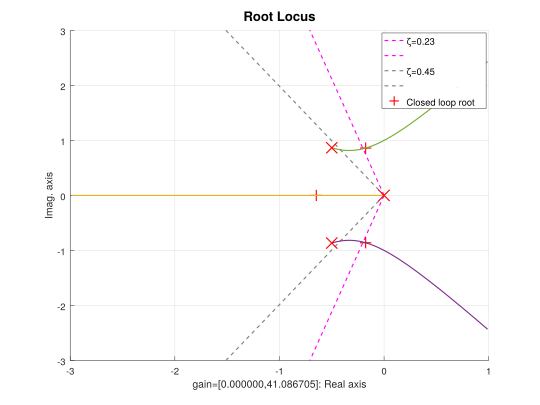
\includegraphics[scale=0.75]{./figuras/chapter_glc/fig_ejem32_GH_ltitool.png}
	\caption{Root locus diagram of Exam. 3.2.}
	\label{chp_lc_fig_LR_ejemGH}
\end{figure}
%\end{example}



\vspace{0.4cm}
\textbf{Ejemplo 3.3}
%\begin{example} \label{ejem03_gh_oct}

Figure \ref{chp_lc_fig01_ejemGH} shows the application window performed for the analysis of closed-loop LTI systems based on the expression of \textit{G}(\textit{s})\textit{H}(\textit{s}).
\begin{figure}[H]
	\centering
	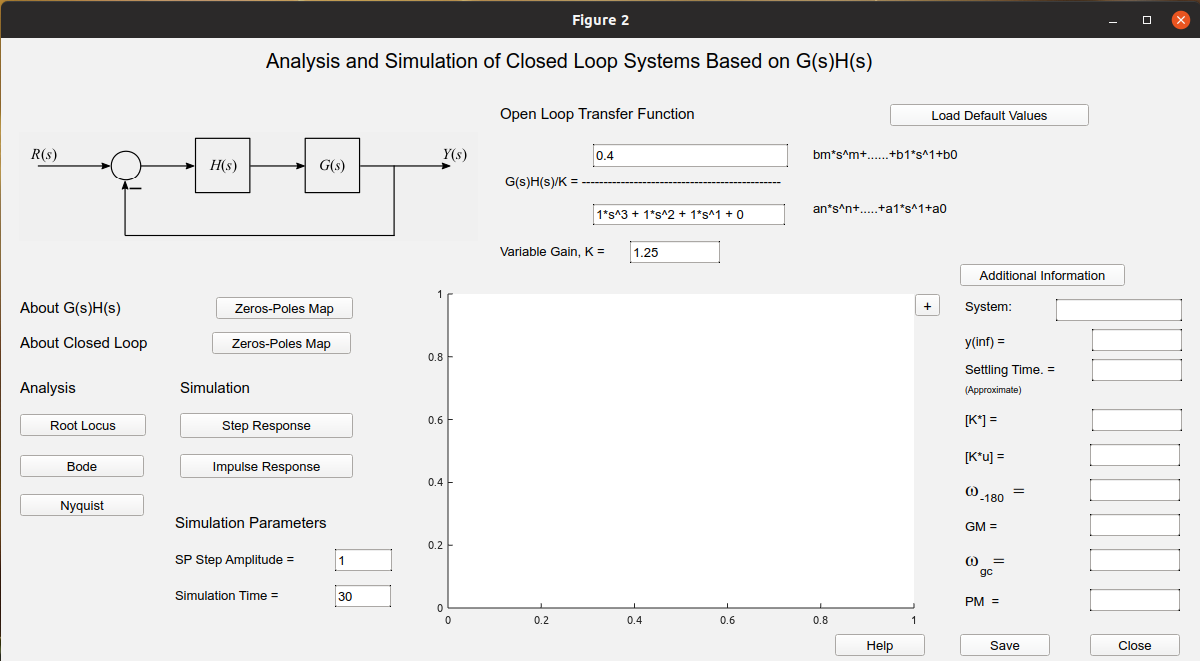
\includegraphics[scale=0.5]{./figuras/chapter_glc/fig01_ejemGH.png}
	\caption{Closed loop system analysis and simulation window based on \textit{G}(\textit{s})\textit{H}(\textit{s}) with preloaded data.}
	\label{chp_lc_fig01_ejemGH}
\end{figure}
Note that the data has been preloaded by a file that saves the data from the last time you worked with this application. There is also a button (Load Default Values Botton) that load the preloaded data for this particular example, which if it pressed, default values are reloaded.

Figure \ref{chp_lc_fig02_ejemGH} shows the numerical simulation of the feedback system when $K^* = 0.5$. Similarly, the poles and zeros maps of \textit{G}(\textit{s})\textit{H}(\textit{s}) can be obtained from the feedback system, together the root locus, Bode and Nyquist diagrams.

In addition, the additional information button provides information of the feedback system related to stability, establishment value, and establishment time, \textit{GM}, \textit{PM}, $\omega_{-180}$ y $\omega_{cg}$. Note that the values $K^*$ and \textit{GM} here reported are coincident with that it was presented by the Exam. 3.1.

\begin{figure}[H]
	\centering
	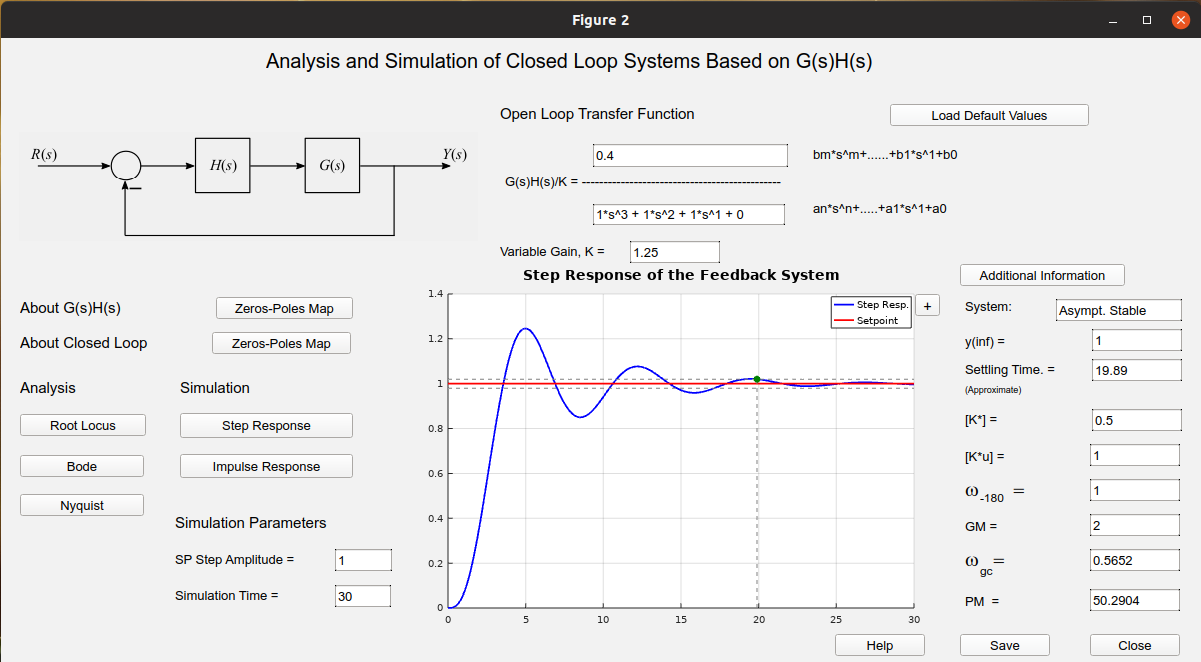
\includegraphics[scale=0.5]{./figuras/chapter_glc/fig02_ejemGH.png}
	\caption{Closed loop system analysis and simulation window based on \textit{G}(\textit{s})\textit{H}(\textit{s}) with step response.}
	\label{chp_lc_fig02_ejemGH}
\end{figure}
%\end{example}





\subsection{Analysis and Simulation of Feedback System}
In this subsection, it will be considered the closed loop system of Fig. \ref{chpCLfig01Gcl}.


\textbf{Example 3.4}

Figure \ref{chp_lc_fig01_Gcl} shows the developed window for analysis and simulation of closed loop system.

\begin{figure}[H]
	\centering
	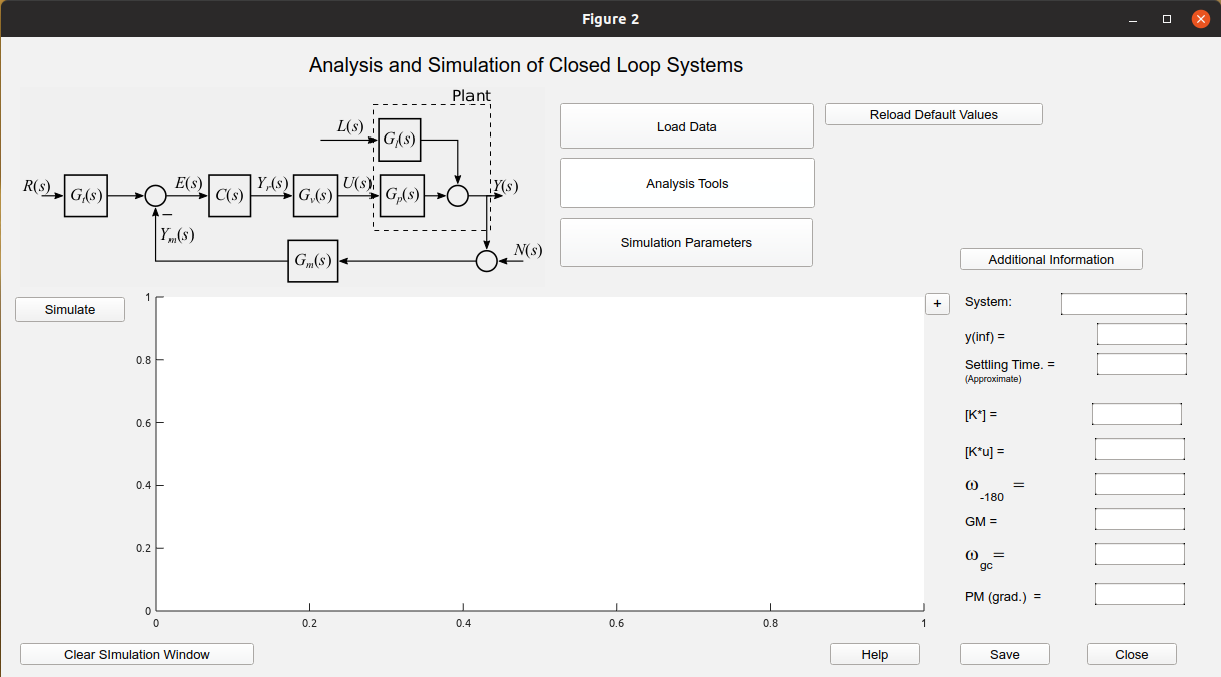
\includegraphics[scale=0.5]{./figuras/chapter_glc/fig01_ejemGcl.png}
	\caption{Main window for analysis and simulation of closed loop system.}
	\label{chp_lc_fig01_Gcl}
\end{figure}

Notice that, if the user press load data button then a window like the one in the Fig. \ref{chp_lc_fig02_Gcl} will be present. In it, the data corresponding to the Fig. \ref{chpCLfig01Gcl} must be loaded.


\begin{figure}[H]
	\centering
	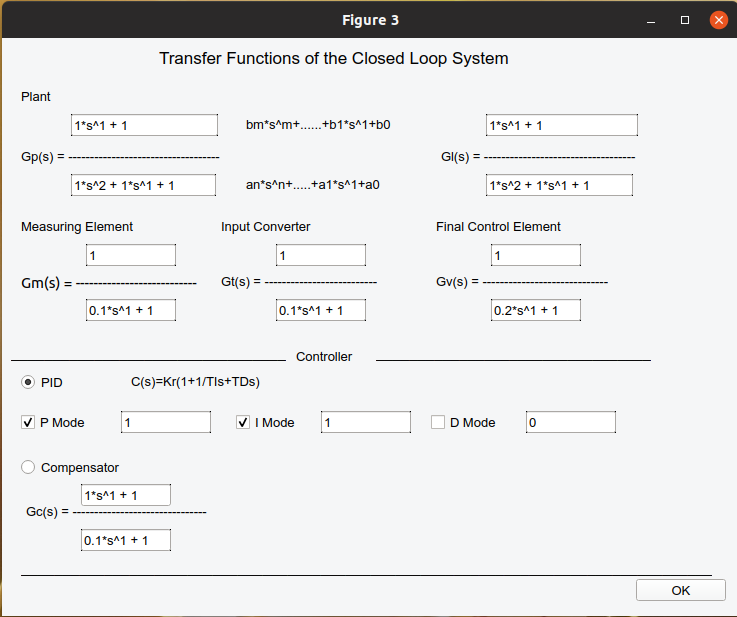
\includegraphics[scale=0.5]{./figuras/chapter_glc/fig02_ejemGcl.png}
	\caption{Window for defining of feedback system transfer function.}
	\label{chp_lc_fig02_Gcl}
\end{figure}

On the other hand, the user has a tool for analysis of feedback systems, if the analysis tools button is pressed. Based on the preloaded data in the previous window, this tool provides in a single window with
\begin{enumerate}
	\item Poles-Zeros Map of \textit{G}(\textit{s})\textit{H}(\textit{s}).
	\item Poles-Zeros Map of the feedback system.
	\item Root locus plot
	\item Bode and Nyquist diagrams
\end{enumerate}
as it is shown in Fig. \ref{chp_lc_fig03_Gcl}.

\begin{figure}[H]
	\centering
	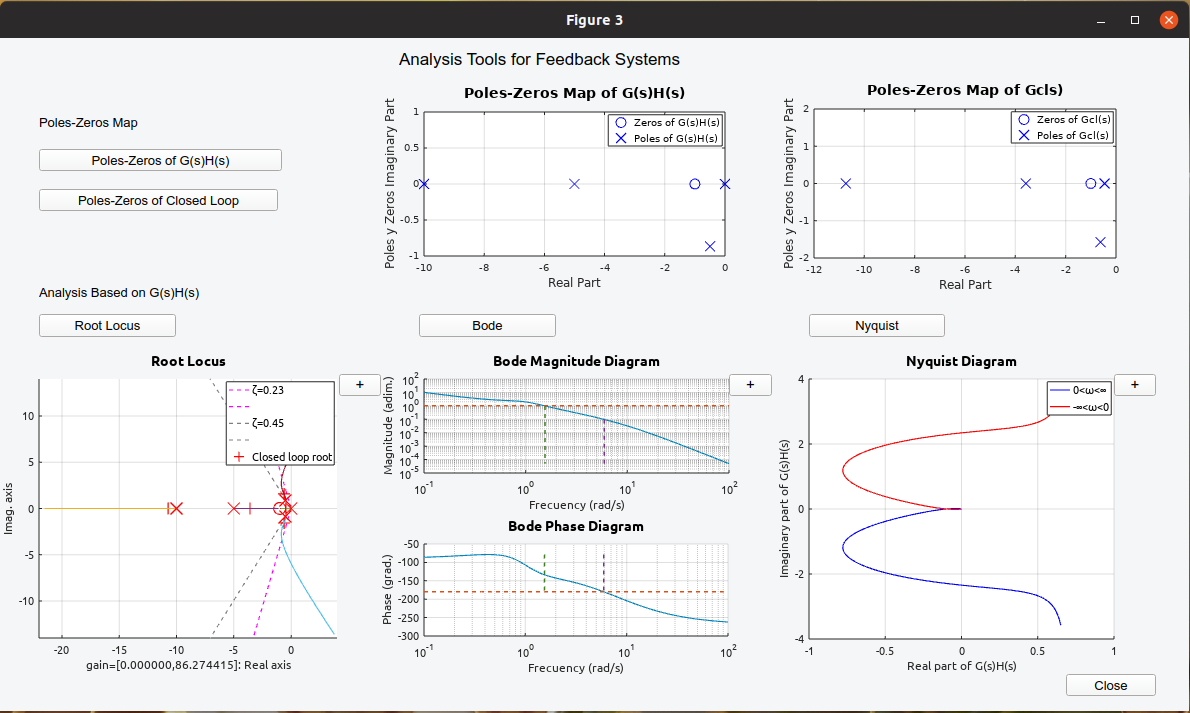
\includegraphics[scale=0.5]{./figuras/chapter_glc/fig03_ejemGcl.png}
	\caption{Tool Window for analysis of feedback system.}
	\label{chp_lc_fig03_Gcl}
\end{figure}

Furthermore, the user has a simulation parameter window where allows setting step amplitude and initial time of set-point and disturbance changes and, the simulation time.

\begin{figure}[H]
	\centering
	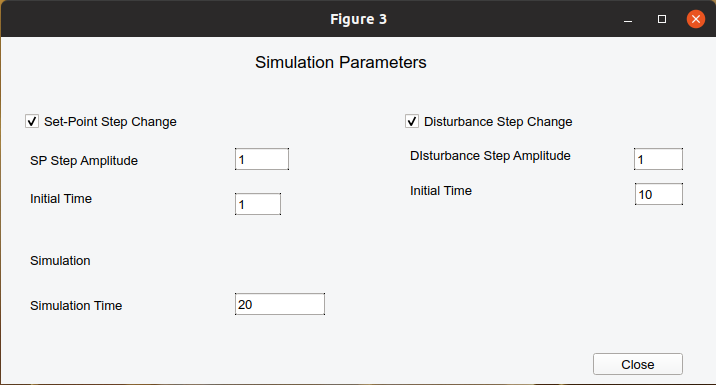
\includegraphics[scale=0.5]{./figuras/chapter_glc/fig04_ejemGcl.png}
	\caption{Tool window for defining simulation parameters.}
	\label{chp_lc_fig04_Gcl}
\end{figure}


Finally, in Fig. \ref{chp_lc_fig05_Gcl} the simulation of this example is shown.

\begin{figure}[H]
	\centering
	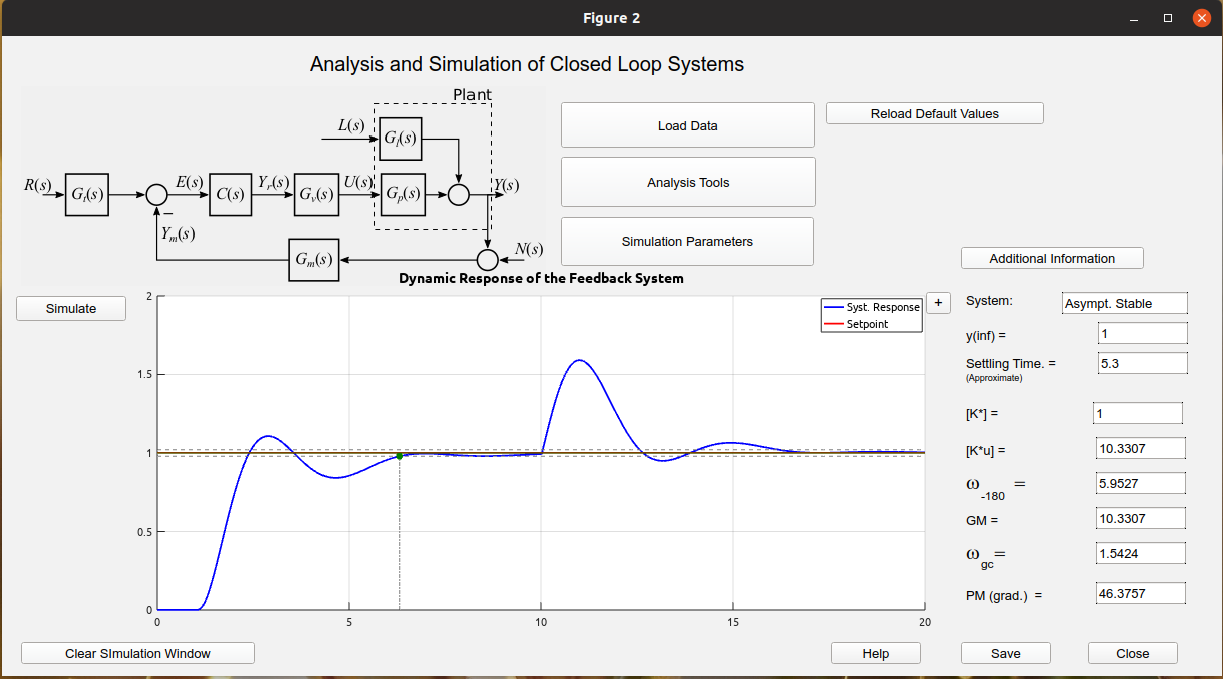
\includegraphics[scale=0.5]{./figuras/chapter_glc/fig05_ejemGcl.png}
	\caption{Window with a simulation example.}
	\label{chp_lc_fig05_Gcl}
\end{figure}


\section{Conclusions}

				% Sistemas a Lazo Cerrado

\chapter{Traditional Advanced Control Strategies} \label{eca_chapter}
%\thispagestyle{fancy}

This chapter presents tools for the analysis and simulation of traditional advanced control strategies such as feedforward-feedback control, cascade control, among others that are currently under development.


\section{Feedforward-Feedback Control}

Consider el feedforward-feedback control system according to Fig. \ref{chp_eca_fig01_ff}.

\begin{figure}[H]
	\centering
	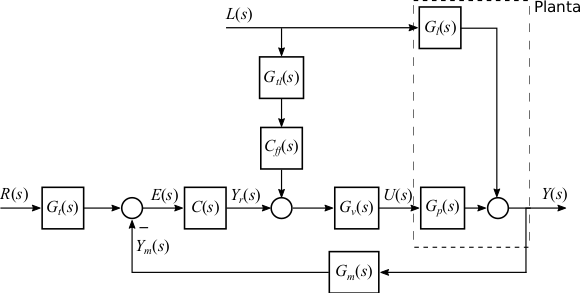
\includegraphics[scale=1.2]{./figuras/chapter_eca/controlFFFB.png}
	\caption{Feedforward-feedback control system.}
	\label{chp_eca_fig01_ff}
\end{figure}




\section{Cascade Control}

Consider the cascade control system according to Fig. \ref{chp_eca_fig01_ccd}.

\begin{figure}[H]
	\centering
	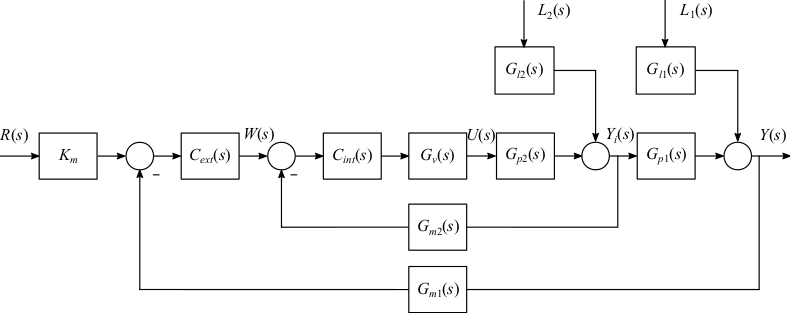
\includegraphics[scale=1.2]{./figuras/chapter_eca/controlCCD.png}
	\caption{Cascade control system.}
	\label{chp_eca_fig01_ccd}
\end{figure}



\section{Tools for Traditional Advanced Control Strategies}

\subsection{Analysis and Simulation of a Feedforward-Feedback Control System}

\textbf{Example 5.1}

Figure \ref{chpECA_fig01_ejemECA} shows the developed main window for traditional advanced control strategies that includes feedforward-feedback control and cascade control schemes.

\begin{figure}[H]
	\centering
	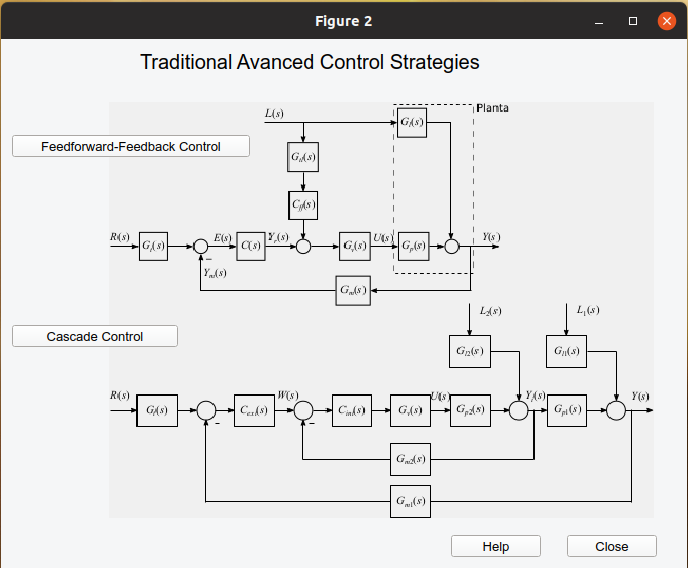
\includegraphics[scale=0.5]{./figuras/chapter_eca/fig01EjemECA.png}
	\caption{Main window for Traditional Advanced Control Strategies.}
	\label{chpECA_fig01_ejemECA}
\end{figure}

Figure \ref{chpECA_fig02_ejemECA} shows the developed main window to study the combined control scheme known as feedforward-feedback control.
\begin{figure}[H]
	\centering
	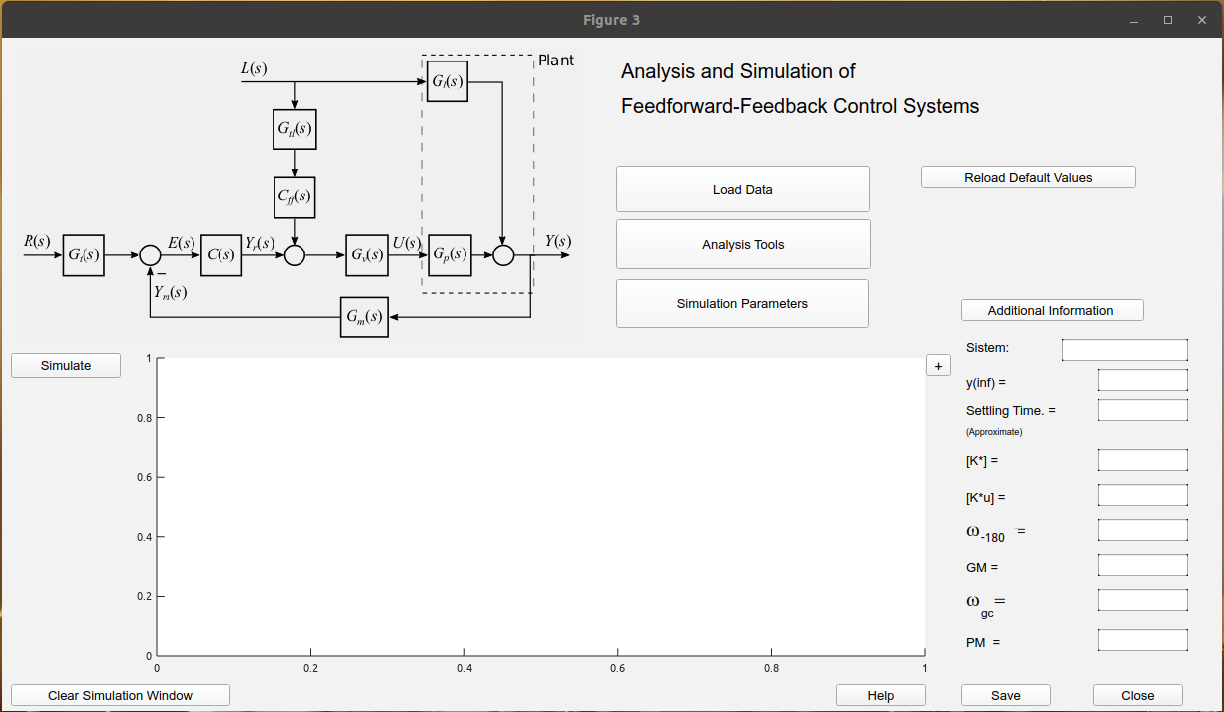
\includegraphics[scale=0.5]{./figuras/chapter_eca/fig02EjemECA.png}
	\caption{Main window for feedforward-feedback control.}
	\label{chpECA_fig02_ejemECA}
\end{figure}

Note that the load data bottom opens a window to load data for this example and it is similar to Fig. \ref{chp_lc_fig02_Gcl}.

Figure \ref{chpECA_fig03_ejemECA} shows the developed analysis tool window which is similar to developed window for closed loop system (Fig. \ref{chp_lc_fig03_Gcl}).
\begin{figure}[H]
	\centering
	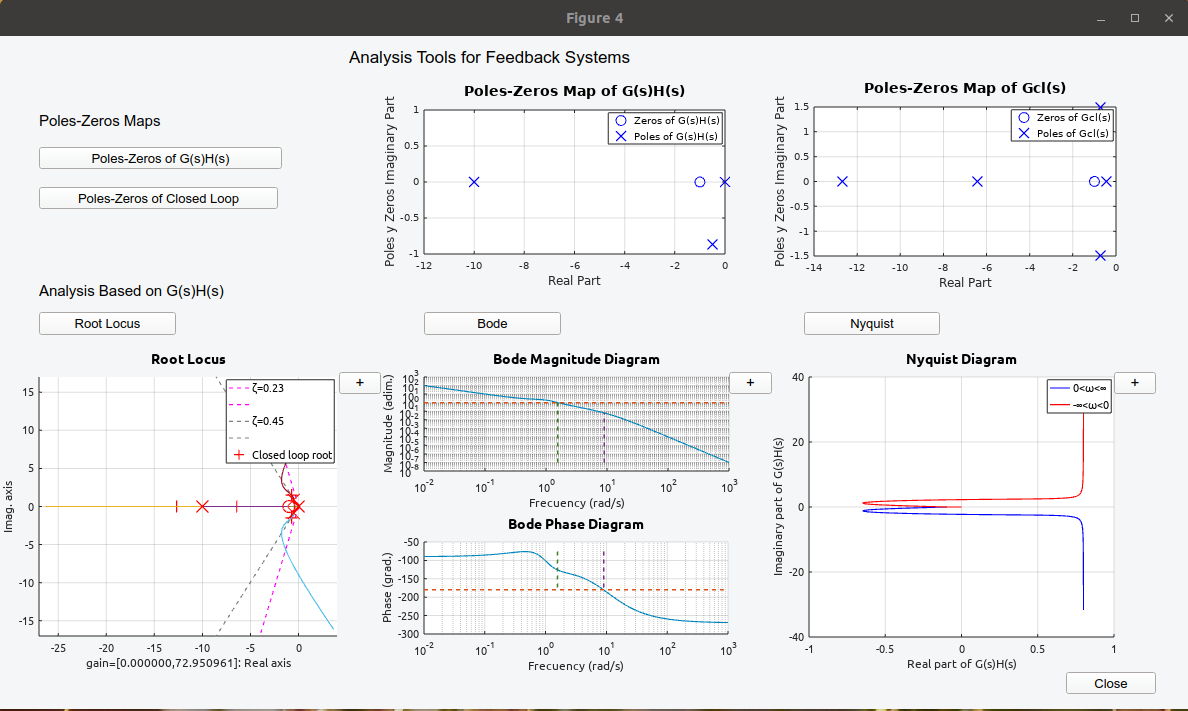
\includegraphics[scale=0.5]{./figuras/chapter_eca/fig03EjemECA.png}
	\caption{Analysis tool window for feedforward-feedback control system.}
	\label{chpECA_fig03_ejemECA}
\end{figure}

Finally, Fig. \ref{chpECA_fig04_ejemECA} shows the simulations obtained with this example.
\begin{figure}[H]
	\centering
	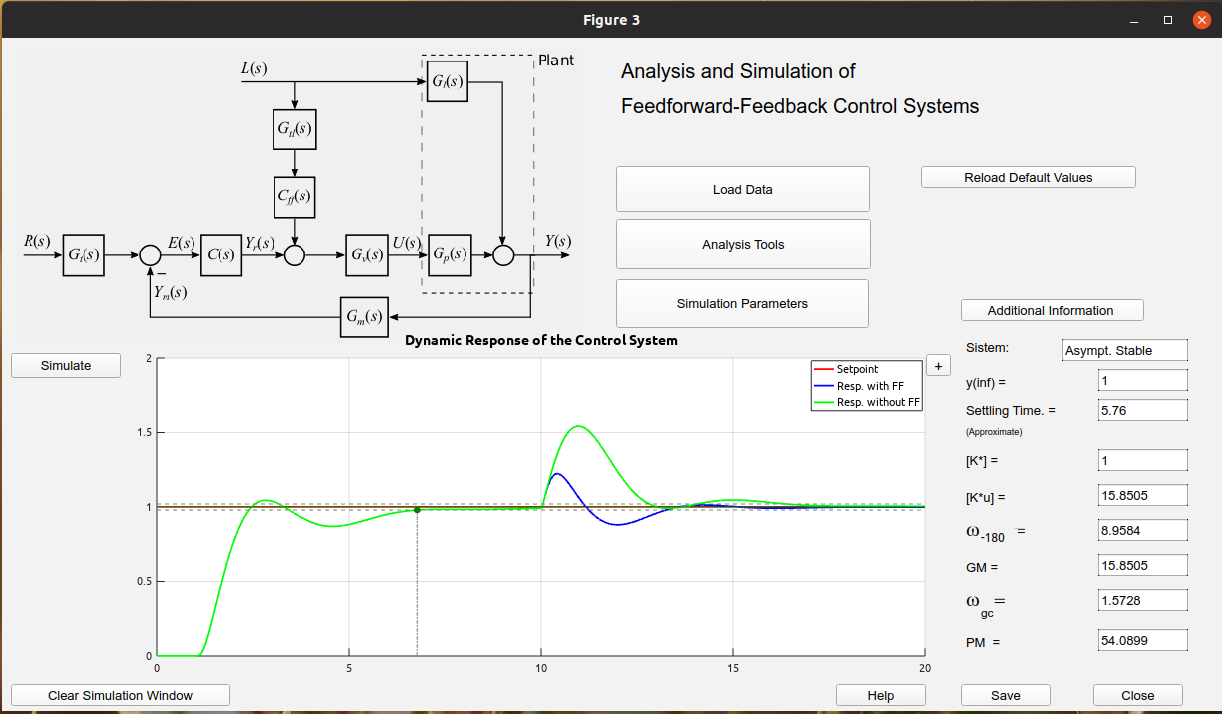
\includegraphics[scale=0.5]{./figuras/chapter_eca/fig04EjemECA.png}
	\caption{Simulation of feedforward-feedback control example.}
	\label{chpECA_fig04_ejemECA}
\end{figure}


\subsection{Analysis and Simulation of a Cascade Control System}

\textbf{Example 5.2}

If the user press the cascade control bottom indicated in Fig. \ref{chpECA_fig01_ejemECA} then, a window developed for cascade control scheme is opened. Figure \ref{chpECA_fig05_ejemECA} shows the developed main window to study this combined control scheme.

\begin{figure}[H]
	\centering
	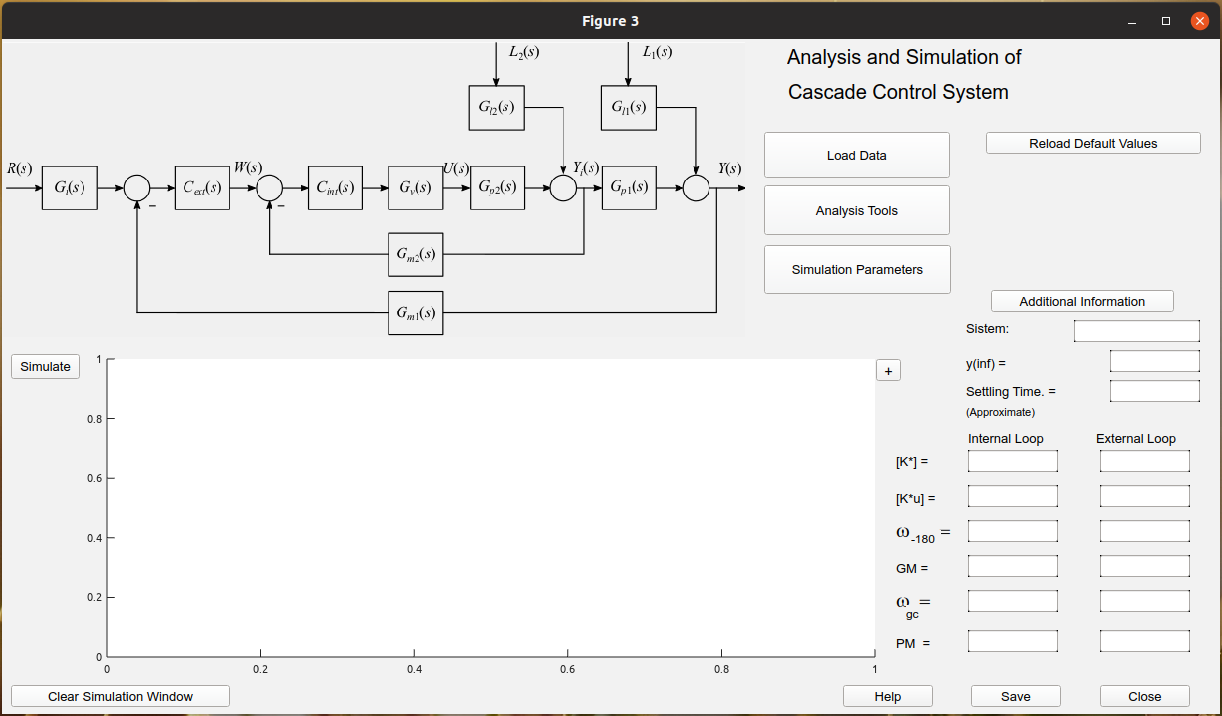
\includegraphics[scale=0.5]{./figuras/chapter_eca/fig05EjemECA.png}
	\caption{Main window for cascade control.}
	\label{chpECA_fig05_ejemECA}
\end{figure}

Note that the load data bottom opens a window to load data for this example and it is similar to Fig. \ref{chp_lc_fig02_Gcl}. Also, when de bottom analysis tools is pressed the window indicated in Fig. is opened.

\begin{figure}[H]
	\centering
	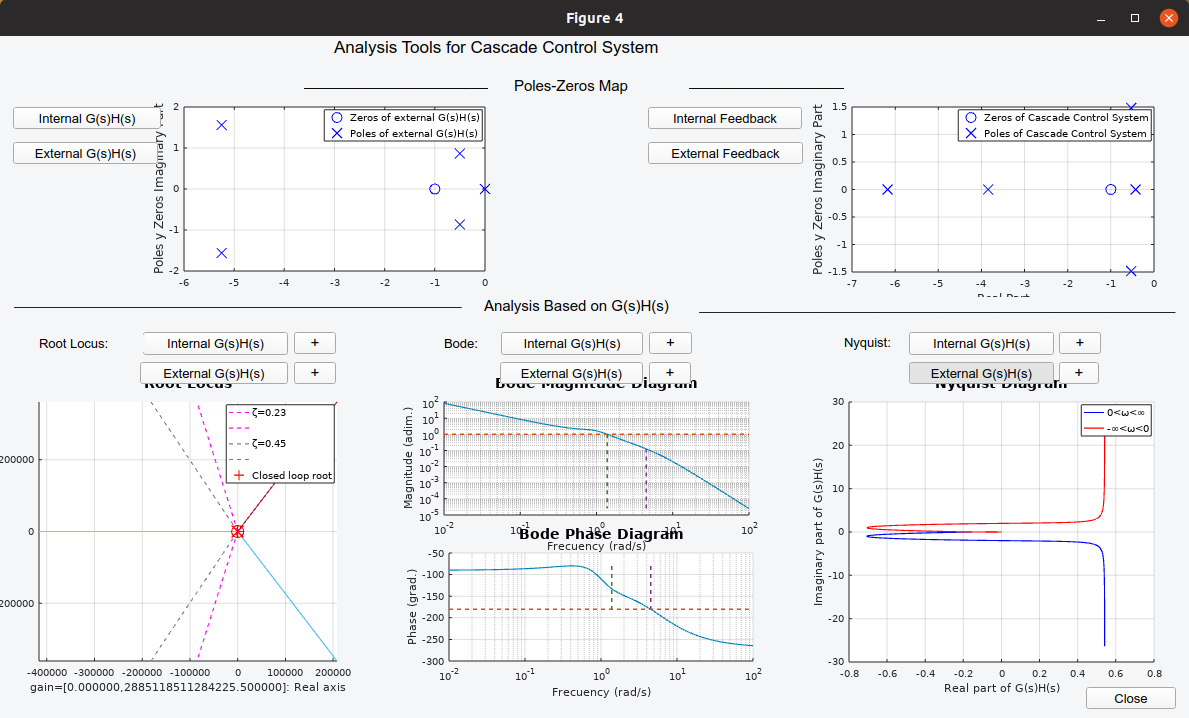
\includegraphics[scale=0.5]{./figuras/chapter_eca/fig06EjemECA.png}
	\caption{Analysis tool window for control control system.}
	\label{chpECA_fig06_ejemECA}
\end{figure}

Note that in mentioned window, the user can study internal and external loop independently.  

Finally, Fig. \ref{chpECA_fig07_ejemECA} shows the simulations obtained with this example.
\begin{figure}[H]
	\centering
	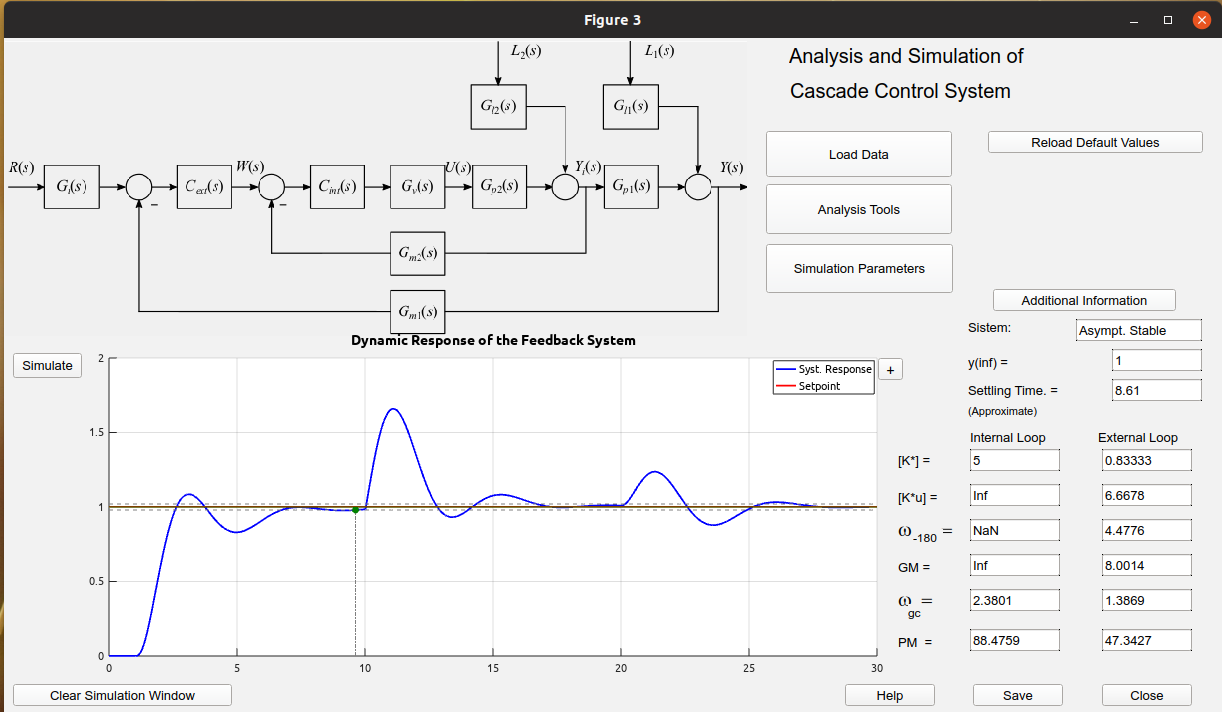
\includegraphics[scale=0.5]{./figuras/chapter_eca/fig07EjemECA.png}
	\caption{Simulation of cascade control example.}
	\label{chpECA_fig07_ejemECA}
\end{figure}


\section{Conclusions}


				% Estrategias de Control Avanzadas
\chapter{Additional Tools for LTI System Control} \label{additool_chapter}


This chapter includes additional tools for LTI system control. These are, Optimal Tuning of  PID Controller, among others that they are in development.

\section{Optimal Setting of PID Controller}

\section{Developed Additional Tools}

\subsection{PID Optimal Controller Setting}

Fig. \ref{chpADDITOOL_fig01_ejemOptimalPID} show the developed main window for tuning PID controller based on mixed criteria. For that, the minimization of ITAE, maximum overshoot and sensitivity function was chosen.


\begin{figure}[H]
	\centering
	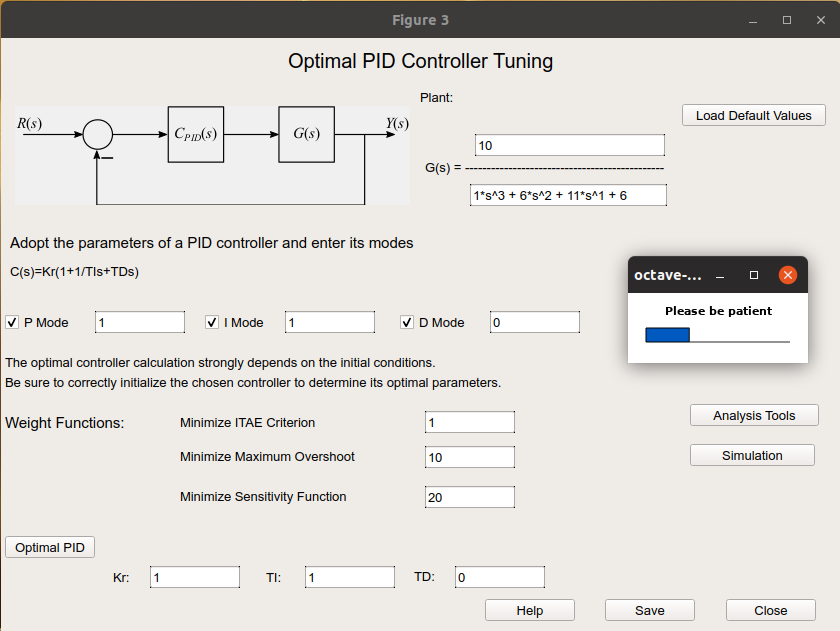
\includegraphics[scale=0.5]{./figuras/chapter_additools/fig01EjemAdditools.png}
	\caption{Main window for tuning optimal PID controllers.}
	\label{chpADDITOOL_fig01_ejemOptimalPID}
\end{figure}

Figure \ref{chpADDITOOL_fig02_ejemOptimalPID} shows simulations an results obtained in this example.
\begin{figure}[H]
	\centering
	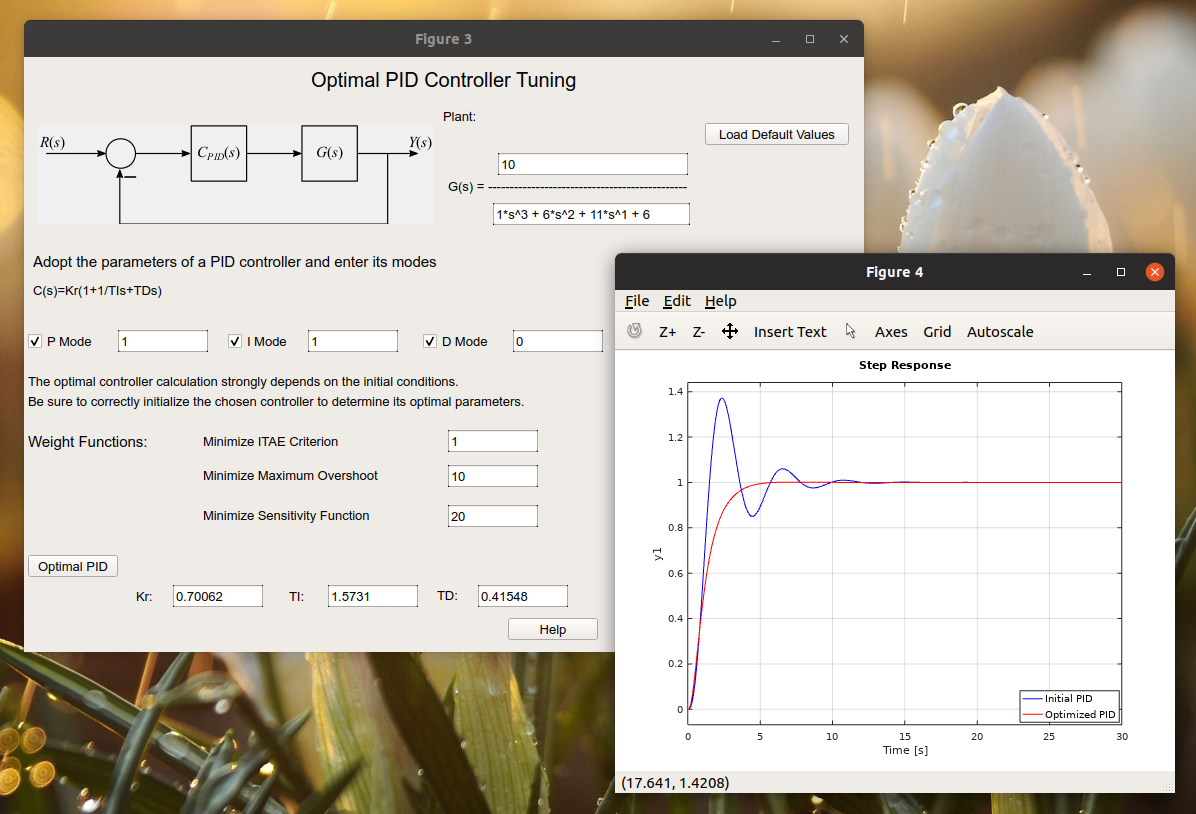
\includegraphics[scale=0.5]{./figuras/chapter_additools/fig02EjemAdditools.png}
	\caption{Comparative simulation between two PID controllers. With color blue it is indicated the simulation with PID controller taken as reference while with color red it corresponds to simulation of optimal PID.}
	\label{chpADDITOOL_fig02_ejemOptimalPID}
\end{figure}





			% Estrategias de Control Avanzadas



\appendix
%A partir de aquí van los apéndices y aparecen todos numerados en el índice.
%\include{appendixA}
%\include{appendixB}

%-----------------------------------------------------------------------


\pagestyle{fancy} 
\fancyhf{} 
\fancyhead{} % Cabecera vacia
\fancyfoot{} %Pie vacio
\renewcommand{\headrulewidth}{0pt}

\printindex % aquí se imprime el índice alfabético

%-----------------------------------------------------------------------


\bibliographystyle{plain}
%\bibliographystyle{alpha}
\bibliography{book_references}

%\begin{thebibliography}{a}
%	\bibitem{Adam2018} 
%		\textsc{E. J. Adam},
%		\textit{Instrumentaci\'on y Control de Procesos. Notas de Clase.},
%		3rd. Ediciones UNL, ISBN 978-987-749-122-7,
%		2018.
%		%bibitem{Dan} \textsc{Dantzig, G.B.} y \textsc{P. Wolfe},<<Decomposition principle for linear programs>>,\textit{Operations Research}, \textbf{8}, págs. 101--111, 1960
%\end{thebibliography}

\end{document}

